% This article has been prepared for publication in Energy Economics in RStudio with knitr.
% According to http://www.elsevier.com/author-schemas/the-elsarticle-latex-document-class, we should be using the
% elsarticle.cls file.
% According to http://cdn.elsevier.com/assets/pdf_file/0006/109392/journal_refstyles.pdf, we should be using
% elsarticle-template-2-harv.tex as the template for the text.
% Furthermore, we should be using model2-names.bst for the bibliographic references.
% The approach here is to load the frontmatter and backmatter from elsarticle-template-2-harv.tex
% both ahead of and behind the text for our paper.
% -- Matthew Kuperus Heun, 2013-01-18

%% This is file `elsarticle-template-2-harv.tex',
%%
%% Copyright 2009 Elsevier Ltd
%%
%% This file is part of the 'Elsarticle  Bundle'.
%% ---------------------------------------------
%%
%% It may be distributed under the conditions of the LaTeX Project Public
%% License, either version 1.2 of this license or (at your option) any
%% later version.  The latest version of this license is in
%%    http://www.latex-project.org/lppl.txt
%% and version 1.2 or later is part of all distributions of LaTeX
%% version 1999/12/01 or later.
%%
%% The list of all files belonging to the 'Elsarticle Bundle' is
%% given in the file `manifest.txt'.
%%
%% Template article for Elsevier's document class `elsarticle'
%% with harvard style bibliographic references
%%
%% $Id: elsarticle-template-2-harv.tex 155 2009-10-08 05:35:05Z rishi $
%% $URL: http://lenova.river-valley.com/svn/elsbst/trunk/elsarticle-template-2-harv.tex $
%%
\documentclass[preprint,authoryear,12pt]{elsarticle}\usepackage{graphicx, color}
%% maxwidth is the original width if it is less than linewidth
%% otherwise use linewidth (to make sure the graphics do not exceed the margin)
\makeatletter
\def\maxwidth{ %
  \ifdim\Gin@nat@width>\linewidth
    \linewidth
  \else
    \Gin@nat@width
  \fi
}
\makeatother

\IfFileExists{upquote.sty}{\usepackage{upquote}}{}
\definecolor{fgcolor}{rgb}{0.2, 0.2, 0.2}
\newcommand{\hlnumber}[1]{\textcolor[rgb]{0,0,0}{#1}}%
\newcommand{\hlfunctioncall}[1]{\textcolor[rgb]{0.501960784313725,0,0.329411764705882}{\textbf{#1}}}%
\newcommand{\hlstring}[1]{\textcolor[rgb]{0.6,0.6,1}{#1}}%
\newcommand{\hlkeyword}[1]{\textcolor[rgb]{0,0,0}{\textbf{#1}}}%
\newcommand{\hlargument}[1]{\textcolor[rgb]{0.690196078431373,0.250980392156863,0.0196078431372549}{#1}}%
\newcommand{\hlcomment}[1]{\textcolor[rgb]{0.180392156862745,0.6,0.341176470588235}{#1}}%
\newcommand{\hlroxygencomment}[1]{\textcolor[rgb]{0.43921568627451,0.47843137254902,0.701960784313725}{#1}}%
\newcommand{\hlformalargs}[1]{\textcolor[rgb]{0.690196078431373,0.250980392156863,0.0196078431372549}{#1}}%
\newcommand{\hleqformalargs}[1]{\textcolor[rgb]{0.690196078431373,0.250980392156863,0.0196078431372549}{#1}}%
\newcommand{\hlassignement}[1]{\textcolor[rgb]{0,0,0}{\textbf{#1}}}%
\newcommand{\hlpackage}[1]{\textcolor[rgb]{0.588235294117647,0.709803921568627,0.145098039215686}{#1}}%
\newcommand{\hlslot}[1]{\textit{#1}}%
\newcommand{\hlsymbol}[1]{\textcolor[rgb]{0,0,0}{#1}}%
\newcommand{\hlprompt}[1]{\textcolor[rgb]{0.2,0.2,0.2}{#1}}%

\usepackage{framed}
\makeatletter
\newenvironment{kframe}{%
 \def\at@end@of@kframe{}%
 \ifinner\ifhmode%
  \def\at@end@of@kframe{\end{minipage}}%
  \begin{minipage}{\columnwidth}%
 \fi\fi%
 \def\FrameCommand##1{\hskip\@totalleftmargin \hskip-\fboxsep
 \colorbox{shadecolor}{##1}\hskip-\fboxsep
     % There is no \\@totalrightmargin, so:
     \hskip-\linewidth \hskip-\@totalleftmargin \hskip\columnwidth}%
 \MakeFramed {\advance\hsize-\width
   \@totalleftmargin\z@ \linewidth\hsize
   \@setminipage}}%
 {\par\unskip\endMakeFramed%
 \at@end@of@kframe}
\makeatother

\definecolor{shadecolor}{rgb}{.97, .97, .97}
\definecolor{messagecolor}{rgb}{0, 0, 0}
\definecolor{warningcolor}{rgb}{1, 0, 1}
\definecolor{errorcolor}{rgb}{1, 0, 0}
\newenvironment{knitrout}{}{} % an empty environment to be redefined in TeX

\usepackage{alltt}

%% Use the option review to obtain double line spacing
%% \documentclass[authoryear,preprint,review,12pt]{elsarticle}

%% Use the options 1p,twocolumn; 3p; 3p,twocolumn; 5p; or 5p,twocolumn
%% for a journal layout:
%% \documentclass[final,authoryear,1p,times]{elsarticle}
%% \documentclass[final,authoryear,1p,times,twocolumn]{elsarticle}
%% \documentclass[final,authoryear,3p,times]{elsarticle}
%% \documentclass[final,authoryear,3p,times,twocolumn]{elsarticle}
%% \documentclass[final,authoryear,5p,times]{elsarticle}
%% \documentclass[final,authoryear,5p,times,twocolumn]{elsarticle}

%% if you use PostScript figures in your article
%% use the graphics package for simple commands
%% \usepackage{graphics}
%% or use the graphicx package for more complicated commands
%% \usepackage{graphicx}
%% or use the epsfig package if you prefer to use the old commands
%% \usepackage{epsfig}

%% The amssymb package provides various useful mathematical symbols
\usepackage{amssymb}
%% The amsthm package provides extended theorem environments
%% \usepackage{amsthm}

%% The lineno packages adds line numbers. Start line numbering with
%% \begin{linenumbers}, end it with \end{linenumbers}. Or switch it on
%% for the whole article with \linenumbers after \end{frontmatter}.
%% \usepackage{lineno}

%% natbib.sty is loaded by default. However, natbib options can be
%% provided with \biboptions{...} command. Following options are
%% valid:

%%   round  -  round parentheses are used (default)
%%   square -  square brackets are used   [option]
%%   curly  -  curly braces are used      {option}
%%   angle  -  angle brackets are used    <option>
%%   semicolon  -  multiple citations separated by semi-colon (default)
%%   colon  - same as semicolon, an earlier confusion
%%   comma  -  separated by comma
%%   authoryear - selects author-year citations (default)
%%   numbers-  selects numerical citations
%%   super  -  numerical citations as superscripts
%%   sort   -  sorts multiple citations according to order in ref. list
%%   sort&compress   -  like sort, but also compresses numerical citations
%%   compress - compresses without sorting
%%   longnamesfirst  -  makes first citation full author list
%%
%% \biboptions{longnamesfirst,comma}

% \biboptions{}

\journal{Energy Economics}

\begin{document}

\begin{frontmatter}

%% Title, authors and addresses

%% use the tnoteref command within \title for footnotes;
%% use the tnotetext command for the associated footnote;
%% use the fnref command within \author or \address for footnotes;
%% use the fntext command for the associated footnote;
%% use the corref command within \author for corresponding author footnotes;
%% use the cortext command for the associated footnote;
%% use the ead command for the email address,
%% and the form \ead[url] for the home page:
%%
%% \title{Title\tnoteref{label1}}
%% \tnotetext[label1]{}
%% \author{Name\corref{cor1}\fnref{label2}}
%% \ead{email address}
%% \ead[url]{home page}
%% \fntext[label2]{}
%% \cortext[cor1]{}
%% \address{Address\fnref{label3}}
%% \fntext[label3]{}

\title{Empirical Analysis of the Role of Energy in Economic Growth}

%% use optional labels to link authors explicitly to addresses:
%% \author[label1,label2]{<author name>}
%% \address[label1]{<address>}
%% \address[label2]{<address>}

\author[Calvin]{Caleb Reese}
\author[Calvin]{Lucas Timmer}
\author[Calvin]{Matthew Kuperus Heun\corref{cor1}}
\ead{mkh2@calvin.edu, tel: +1 (616) 526-6663, fax: +1 (616) 526-6501}

\cortext[cor1]{Corresponding author}
\address[Calvin]{Engineering Department, Calvin College, Grand Rapids, MI 49546, USA}

\begin{abstract}
%% Text of abstract
*********** Add abstract ***********
\end{abstract}

\begin{keyword}
%% keywords here, in the form: keyword \sep keyword
economic growth \sep energy \sep cobb-douglas \sep CES \sep LINEX
%% MSC codes here, in the form: \MSC code \sep code
%% or \MSC[2008] code \sep code (2000 is the default)
\end{keyword}

\end{frontmatter}

% \linenumbers
%% main text

Caleb, put your LaTeX code here.











\begin{knitrout}
\definecolor{shadecolor}{rgb}{0.969, 0.969, 0.969}\color{fgcolor}\begin{figure}[]

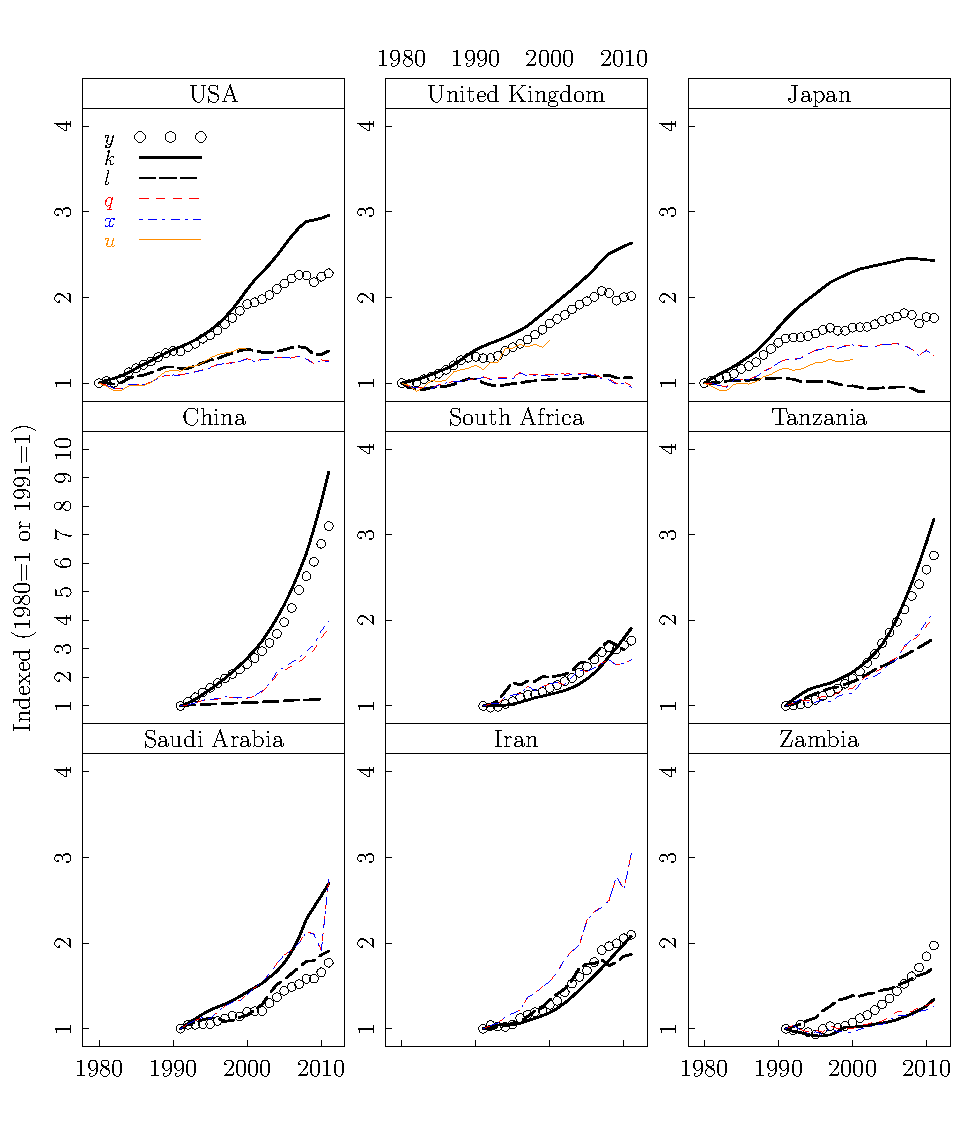
\includegraphics[width=\maxwidth]{figure/Factors_Lattice_Graph} \caption[GDP ($y$), capital stock ($k$), labor ($l$), thermal energy ($q$), exergy ($x$), and useful work ($u$) for all economies]{GDP ($y$), capital stock ($k$), labor ($l$), thermal energy ($q$), exergy ($x$), and useful work ($u$) for all economies. (China's indexed GDP and indexed capital stock rise to $y = 7.3$ and $k = 9.2$ in 2011.)\label{fig:Factors_Lattice_Graph}}
\end{figure}


\end{knitrout}


\section{Cobb-Douglas Without Energy}




% latex table generated in R 2.15.2 by xtable 1.7-0 package
% Wed Jan 30 20:56:18 2013
\begin{table}[ht]
\begin{center}
\caption{Cobb-Douglas parameters for 1980-2011 (US, UK, JP) or 1991-2011 (others). (Parameter estimates beneath symbol. 95\% confidence bounds to left and right.)}
\begin{tabular}{r|ccc|ccc|ccc}
  \hline
 &   & $\lambda$ &   &   & $\alpha$ &   &   & $\beta$ &   \\ 
  \hline
US & 0.0087 & 0.0102 & 0.0116 & 0.21 & 0.27 & 0.34 & 0.66 & 0.73 & 0.79 \\ 
  UK & -0.0104 & 0.0097 & 0.0303 & -0.25 & 0.44 & 1.12 & -0.13 & 0.56 & 1.24 \\ 
  JP & 0.0021 & 0.0052 & 0.0082 & 0.44 & 0.52 & 0.59 & 0.41 & 0.48 & 0.56 \\ 
  CN & -0.0405 & 0.0188 & 0.0779 & 0.11 & 0.71 & 1.32 & -0.32 & 0.29 & 0.89 \\ 
  ZA & -0.0007 & 0.0008 & 0.0022 & 0.46 & 0.60 & 0.73 & 0.26 & 0.40 & 0.54 \\ 
  SA & -0.0159 & -0.0123 & -0.0087 & 0.21 & 0.45 & 0.68 & 0.32 & 0.55 & 0.78 \\ 
  IR & 0.0032 & 0.0039 & 0.0045 & 0.49 & 0.60 & 0.70 & 0.30 & 0.40 & 0.51 \\ 
  TZ & -0.0039 & 0.0015 & 0.0068 & 0.50 & 0.73 & 0.95 & 0.05 & 0.27 & 0.50 \\ 
  ZM & 0.0218 & 0.0249 & 0.0280 & 1.25 & 1.41 & 1.57 & -0.57 & -0.41 & -0.25 \\ 
   \hline
\end{tabular}
\end{center}
\end{table}



\begin{knitrout}
\definecolor{shadecolor}{rgb}{0.969, 0.969, 0.969}\color{fgcolor}\begin{kframe}
\begin{alltt}
usModel <- \hlfunctioncall{cobbDouglasModel}(\hlstring{"US"})
coefs <- \hlfunctioncall{coef}(usModel)
\hlcomment{# print(coef(usModel))}
usPred <- \hlfunctioncall{predict}(usModel) \hlcomment{#See http://stackoverflow.com/questions/9918807/how-get-plot-from-nls-in-r}
\hlfunctioncall{class}(usPred)
\end{alltt}
\begin{verbatim}
[1] "numeric"
\end{verbatim}
\begin{alltt}
\hlcomment{#print(usPred)}
\hlfunctioncall{data.frame}(usPred)
\end{alltt}
\begin{verbatim}
   usPred
1   1.000
2   1.021
3   1.026
4   1.057
5   1.119
6   1.162
7   1.196
8   1.244
9   1.296
10  1.348
11  1.375
12  1.383
13  1.408
14  1.458
15  1.520
16  1.579
17  1.628
18  1.702
19  1.772
20  1.844
21  1.912
22  1.941
23  1.963
24  1.997
25  2.058
26  2.128
27  2.204
28  2.260
29  2.281
30  2.215
31  2.241
32  2.323
\end{verbatim}
\begin{alltt}

allData <- \hlfunctioncall{loadData}(\hlstring{"All"})
predictions <- \hlfunctioncall{cobbDouglasPredictionsColumn}()
\end{alltt}
\begin{verbatim}
    predGDP
1    1.0000
2    1.0206
3    1.0260
4    1.0574
5    1.1188
6    1.1617
7    1.1960
8    1.2438
9    1.2959
10   1.3479
11   1.3747
12   1.3831
13   1.4078
14   1.4579
15   1.5203
16   1.5790
17   1.6283
18   1.7016
19   1.7716
20   1.8440
21   1.9118
22   1.9406
23   1.9632
24   1.9971
25   2.0579
26   2.1281
27   2.2039
28   2.2598
29   2.2806
30   2.2146
31   2.2410
32   2.3234
33   1.0000
34   0.9917
35   0.9988
36   1.0134
37   1.0516
38   1.0850
39   1.1125
40   1.1559
41   1.2165
42   1.2748
43   1.3089
44   1.3079
45   1.3146
46   1.3321
47   1.3702
48   1.4093
49   1.4477
50   1.4962
51   1.5457
52   1.5965
53   1.6418
54   1.6943
55   1.7365
56   1.7840
57   1.8393
58   1.8986
59   1.9551
60   2.0204
61   2.0744
62   2.0753
63   2.1175
64   2.1507
65   1.0000
66   1.0341
67   1.0675
68   1.1023
69   1.1362
70   1.1669
71   1.2030
72   1.2440
73   1.2962
74   1.3463
75   1.4004
76   1.4489
77   1.4862
78   1.5076
79   1.5401
80   1.5772
81   1.6141
82   1.6410
83   1.6477
84   1.6528
85   1.6774
86   1.6836
87   1.6845
88   1.7023
89   1.7261
90   1.7432
91   1.7679
92   1.7838
93   1.7840
94   1.7526
95   1.7641
96   1.7440
97   1.0000
98   1.0975
99   1.2235
100  1.3647
101  1.5167
102  1.6811
103  1.8553
104  2.0466
105  2.2459
106  2.4723
107  2.6961
108  2.9711
109  3.2927
110  3.6207
111  4.0117
112  4.4483
113  4.9207
114  5.4276
115  6.0583
116  6.7711
117  1.0000
118  1.0099
119  1.0264
120  1.0732
121  1.1213
122  1.1238
123  1.1582
124  1.1761
125  1.2075
126  1.2210
127  1.2402
128  1.2634
129  1.2996
130  1.3643
131  1.4082
132  1.4839
133  1.5783
134  1.6682
135  1.7175
136  1.7616
137  1.0000
138  1.0411
139  1.0691
140  1.0932
141  1.1105
142  1.1084
143  1.0905
144  1.0967
145  1.1211
146  1.1406
147  1.1748
148  1.2125
149  1.2863
150  1.3501
151  1.3953
152  1.4590
153  1.5323
154  1.6186
155  1.6435
156  1.6990
157  1.7406
158  1.0000
159  1.0178
160  1.0454
161  1.0538
162  1.0717
163  1.0899
164  1.1390
165  1.1857
166  1.2278
167  1.2926
168  1.3538
169  1.4234
170  1.5165
171  1.6318
172  1.7109
173  1.7735
174  1.8569
175  1.8944
176  1.9799
177  2.0761
178  2.1548
179  1.0000
180  1.0639
181  1.1155
182  1.1713
183  1.2042
184  1.2333
185  1.2610
186  1.2943
187  1.3360
188  1.3816
189  1.4377
190  1.5055
191  1.5879
192  1.6755
193  1.7869
194  1.9203
195  2.0749
196  2.2377
197  2.4150
198  2.6023
199  2.8013
200  1.0000
201  0.9708
202  0.9669
203  0.9380
204  0.9327
205  0.9256
206  0.9514
207  1.0057
208  1.1091
209  1.1221
210  1.1656
211  1.2052
212  1.2585
213  1.2987
214  1.3548
215  1.4198
216  1.4976
217  1.5886
218  1.6883
219  1.8248
220  1.9983
\end{verbatim}
\begin{alltt}
allData <- \hlfunctioncall{cbind}(allData, predictions)
\end{alltt}


{\ttfamily\noindent\bfseries\color{errorcolor}{Error: arguments imply differing number of rows: 222, 220}}\begin{alltt}

\hlfunctioncall{print}(allData)
\end{alltt}
\begin{verbatim}
    Year iYear   iGDP iLabor iCapStk     iQ     iX     iU Country
1   1980     0 1.0000 1.0000  1.0000 1.0000 1.0000 1.0000      US
2   1981     1 1.0254 1.0021  1.0322 0.9768 0.9764 0.9617      US
3   1982     2 1.0055 0.9872  1.0551 0.9389 0.9379 0.9148      US
4   1983     3 1.0509 1.0049  1.0829 0.9337 0.9327 0.9116      US
5   1984     4 1.1264 1.0556  1.1253 0.9799 0.9790 0.9657      US
6   1985     5 1.1730 1.0797  1.1718 0.9790 0.9782 0.9782      US
7   1986     6 1.2137 1.0924  1.2172 0.9818 0.9808 0.9712      US
8   1987     7 1.2525 1.1220  1.2608 1.0134 1.0126 1.0051      US
9   1988     8 1.3040 1.1555  1.3054 1.0590 1.0582 1.0732      US
10  1989     9 1.3506 1.1874  1.3511 1.0915 1.0897 1.1328      US
11  1990    10 1.3759 1.1894  1.3927 1.0973 1.0948 1.1516      US
12  1991    11 1.3727 1.1726  1.4246 1.0970 1.0941 1.1389      US
13  1992    12 1.4193 1.1736  1.4612 1.1126 1.1098 1.1874      US
14  1993    13 1.4598 1.2010  1.5048 1.1340 1.1312 1.1996      US
15  1994    14 1.5192 1.2386  1.5570 1.1561 1.1532 1.2387      US
16  1995    15 1.5574 1.2691  1.6155 1.1816 1.1779 1.2920      US
17  1996    16 1.6157 1.2850  1.6848 1.2200 1.2164 1.3335      US
18  1997    17 1.6877 1.3226  1.7662 1.2303 1.2271 1.3523      US
19  1998    18 1.7612 1.3511  1.8634 1.2384 1.2353 1.3669      US
20  1999    19 1.8462 1.3775  1.9745 1.2584 1.2550 1.4091      US
21  2000    20 1.9226 1.3959  2.0955 1.2848 1.2816 1.3964      US
22  2001    21 1.9434 1.3788  2.2033 1.2548 1.2516     NA      US
23  2002    22 1.9786 1.3609  2.2927 1.2779 1.2739     NA      US
24  2003    23 2.0289 1.3538  2.3844 1.2806 1.2769     NA      US
25  2004    24 2.0992 1.3690  2.4885 1.3018 1.2981     NA      US
26  2005    25 2.1637 1.3901  2.6029 1.3036 1.2997     NA      US
27  2006    26 2.2212 1.4155  2.7162 1.2960 1.2916     NA      US
28  2007    27 2.2637 1.4253  2.8158 1.3178 1.3132     NA      US
29  2008    28 2.2561 1.4099  2.8877 1.2874 1.2819     NA      US
30  2009    29 2.1774 1.3323  2.9041 1.2307 1.2239     NA      US
31  2010    30 2.2434 1.3318  2.9249 1.2710 1.2647     NA      US
32  2011    31 2.2823 1.3742  2.9597 1.2586 1.2508     NA      US
33  1980     0 1.0000 1.0000  1.0000 1.0000 1.0000 1.0000      UK
34  1981     1 0.9868 0.9541  1.0184 0.9607 0.9599 0.9725      UK
35  1982     2 1.0074 0.9334  1.0407 0.9489 0.9473 0.9069      UK
36  1983     3 1.0439 0.9234  1.0663 0.9531 0.9509 0.9521      UK
37  1984     4 1.0718 0.9466  1.0990 0.9374 0.9331 1.0317      UK
38  1985     5 1.1104 0.9598  1.1339 0.9824 0.9789 1.0175      UK
39  1986     6 1.1549 0.9630  1.1687 1.0053 1.0024 1.0315      UK
40  1987     7 1.2076 0.9848  1.2120 1.0173 1.0145 1.1298      UK
41  1988     8 1.2684 1.0214  1.2709 1.0199 1.0161 1.1561      UK
42  1989     9 1.2974 1.0503  1.3343 1.0447 1.0404 1.1731      UK
43  1990    10 1.3075 1.0475  1.3900 1.0496 1.0448 1.2083      UK
44  1991    11 1.2893 1.0051  1.4296 1.0726 1.0676 1.1603      UK
45  1992    12 1.2911 0.9774  1.4653 1.0474 1.0410 1.2362      UK
46  1993    13 1.3198 0.9663  1.4981 1.0593 1.0509 1.2455      UK
47  1994    14 1.3763 0.9798  1.5348 1.0655 1.0563 1.4084      UK
48  1995    15 1.4183 0.9931  1.5732 1.0623 1.0519 1.4071      UK
49  1996    16 1.4593 1.0021  1.6167 1.1283 1.1167 1.4547      UK
50  1997    17 1.5092 1.0190  1.6683 1.0963 1.0838 1.4218      UK
51  1998    18 1.5672 1.0273  1.7385 1.1004 1.0872 1.4527      UK
52  1999    19 1.6244 1.0365  1.8091 1.1026 1.0885 1.4201      UK
53  2000    20 1.6969 1.0389  1.8797 1.0955 1.0815 1.4983      UK
54  2001    21 1.7503 1.0489  1.9506 1.1173 1.1032     NA      UK
55  2002    22 1.7968 1.0460  2.0239 1.1051 1.0904     NA      UK
56  2003    23 1.8602 1.0499  2.0944 1.1122 1.0982     NA      UK
57  2004    24 1.9151 1.0593  2.1707 1.1144 1.1008     NA      UK
58  2005    25 1.9551 1.0720  2.2471 1.1153 1.1017     NA      UK
59  2006    26 2.0061 1.0778  2.3327 1.1029 1.0899     NA      UK
60  2007    27 2.0756 1.0868  2.4320 1.0609 1.0479     NA      UK
61  2008    28 2.0527 1.0914  2.5117 1.0494 1.0360     NA      UK
62  2009    29 1.9629 1.0597  2.5523 0.9990 0.9838     NA      UK
63  2010    30 2.0040 1.0649  2.5969 1.0153 1.0003     NA      UK
64  2011    31 2.0171 1.0634  2.6358 0.9669 0.9518     NA      UK
65  1980     0 1.0000 1.0000  1.0000 1.0000 1.0000 1.0000      JP
66  1981     1 1.0293 1.0030  1.0536 1.0001 0.9998 0.9624      JP
67  1982     2 1.0578 1.0087  1.1034 0.9730 0.9710 0.9176      JP
68  1983     3 1.0748 1.0222  1.1481 0.9547 0.9510 0.9101      JP
69  1984     4 1.1084 1.0319  1.1949 1.0393 1.0367 0.9869      JP
70  1985     5 1.1647 1.0290  1.2489 1.0439 1.0397 0.9950      JP
71  1986     6 1.1992 1.0332  1.3068 1.0464 1.0415 0.9891      JP
72  1987     7 1.2447 1.0400  1.3722 1.0787 1.0734 1.0168      JP
73  1988     8 1.3289 1.0531  1.4539 1.1391 1.1351 1.0744      JP
74  1989     9 1.3992 1.0554  1.5462 1.1774 1.1737 1.1009      JP
75  1990    10 1.4719 1.0587  1.6473 1.2402 1.2371 1.1523      JP
76  1991    11 1.5209 1.0559  1.7466 1.2748 1.2710 1.1769      JP
77  1992    12 1.5333 1.0451  1.8342 1.2783 1.2745 1.1505      JP
78  1993    13 1.5360 1.0200  1.9101 1.2933 1.2881 1.1599      JP
79  1994    14 1.5492 1.0163  1.9775 1.3434 1.3398 1.2008      JP
80  1995    15 1.5791 1.0208  2.0417 1.3836 1.3792 1.2375      JP
81  1996    16 1.6211 1.0223  2.1111 1.4058 1.4013 1.2441      JP
82  1997    17 1.6472 1.0137  2.1754 1.4318 1.4265 1.2796      JP
83  1998    18 1.6125 0.9899  2.2197 1.4101 1.4036 1.2463      JP
84  1999    19 1.6112 0.9669  2.2603 1.4364 1.4317 1.2612      JP
85  2000    20 1.6472 0.9683  2.2994 1.4497 1.4454 1.2732      JP
86  2001    21 1.6530 0.9513  2.3313 1.4360 1.4316     NA      JP
87  2002    22 1.6577 0.9336  2.3517 1.4262 1.4227     NA      JP
88  2003    23 1.6862 0.9356  2.3713 1.4231 1.4213     NA      JP
89  2004    24 1.7256 0.9447  2.3900 1.4564 1.4541     NA      JP
90  2005    25 1.7478 0.9459  2.4089 1.4525 1.4494     NA      JP
91  2006    26 1.7772 0.9547  2.4294 1.4642 1.4602     NA      JP
92  2007    27 1.8157 0.9541  2.4489 1.4436 1.4407     NA      JP
93  2008    28 1.7962 0.9401  2.4587 1.3966 1.3927     NA      JP
94  2009    29 1.6969 0.9005  2.4489 1.3225 1.3155     NA      JP
95  2010    30 1.7726 0.9067  2.4397 1.3873 1.3815     NA      JP
96  2011    31 1.7598     NA  2.4320 1.3182 1.3156     NA      JP
97  1991     0 1.0000 1.0000  1.0000 1.0000 1.0000     NA      CN
98  1992     1 1.1420 1.0258  1.0985 1.0356 1.0366     NA      CN
99  1993     2 1.3019 1.0377  1.2404 1.1039 1.1109     NA      CN
100 1994     3 1.4724 1.0501  1.4015 1.1878 1.2025     NA      CN
101 1995     4 1.6329 1.0615  1.5763 1.2123 1.2276     NA      CN
102 1996     5 1.7962 1.0727  1.7664 1.2396 1.2565     NA      CN
103 1997     6 1.9633 1.0838  1.9675 1.3058 1.3298     NA      CN
104 1998     7 2.1164 1.0944  2.1906 1.2877 1.3073     NA      CN
105 1999     8 2.2772 1.1039  2.4224 1.2716 1.2873     NA      CN
106 2000     9 2.4685 1.1277  2.6767 1.2703 1.2822     NA      CN
107 2001    10 2.6734 1.1206  2.9517 1.3336 1.3521     NA      CN
108 2002    11 2.9167 1.1431  3.2685 1.4993 1.5349     NA      CN
109 2003    12 3.2084 1.1654  3.6489 1.7220 1.7815     NA      CN
110 2004    13 3.5324 1.1563  4.0735 2.0815 2.1830     NA      CN
111 2005    14 3.9316 1.1782  4.5471 2.2471 2.3645     NA      CN
112 2006    15 4.4309 1.2000  5.0820 2.3911 2.5214     NA      CN
113 2007    16 5.0601 1.2063  5.6910 2.5309 2.6764     NA      CN
114 2008    17 5.5458 1.2108  6.3512 2.7533 2.9220     NA      CN
115 2009    18 6.0561 1.2169  7.2033 2.9489 3.1387     NA      CN
116 2010    19 6.6845 1.2381  8.1442 3.3926 3.6274     NA      CN
117 2011    20 7.3013     NA  9.1896 3.7111 3.9776     NA      CN
118 1991     0 1.0000 1.0000  1.0000 1.0000 1.0000     NA      ZA
119 1992     1 0.9786 1.0211  1.0012 1.0229 1.0232     NA      ZA
120 1993     2 0.9907 1.0597  1.0019 1.0228 1.0226     NA      ZA
121 1994     3 1.0227 1.1704  1.0084 1.1113 1.1103     NA      ZA
122 1995     4 1.0546 1.2757  1.0227 1.1294 1.1270     NA      ZA
123 1996     5 1.1000 1.2423  1.0436 1.1437 1.1420     NA      ZA
124 1997     6 1.1291 1.2909  1.0683 1.2329 1.2323     NA      ZA
125 1998     7 1.1350 1.2885  1.0960 1.1784 1.1763     NA      ZA
126 1999     8 1.1617 1.3403  1.1139 1.2262 1.2249     NA      ZA
127 2000     9 1.2100 1.3387  1.1343 1.2584 1.2576     NA      ZA
128 2001    10 1.2431 1.3506  1.1560 1.2739 1.2737     NA      ZA
129 2002    11 1.2887 1.3694  1.1798 1.2477 1.2460     NA      ZA
130 2003    12 1.3267 1.4076  1.2126 1.3375 1.3377     NA      ZA
131 2004    13 1.3871 1.5013  1.2579 1.4192 1.4193     NA      ZA
132 2005    14 1.4603 1.5185  1.3144 1.4029 1.4023     NA      ZA
133 2006    15 1.5422 1.5982  1.3845 1.4428 1.4414     NA      ZA
134 2007    16 1.6268 1.6966  1.4726 1.4988 1.4963     NA      ZA
135 2008    17 1.6866 1.7563  1.5763 1.5387 1.5367     NA      ZA
136 2009    18 1.6613 1.7141  1.6803 1.4780 1.4758     NA      ZA
137 2010    19 1.7095 1.6557  1.7923 1.5004 1.4994     NA      ZA
138 2011    20 1.7625     NA  1.9066 1.5383 1.5402     NA      ZA
139 1991     0 1.0000 1.0000  1.0000 1.0000 1.0000     NA      SA
140 1992     1 1.0463 1.0492  1.0599 1.0553 1.0553     NA      SA
141 1993     2 1.0466 1.0792  1.1165 1.0984 1.0982     NA      SA
142 1994     3 1.0535 1.1059  1.1703 1.1317 1.1313     NA      SA
143 1995     4 1.0556 1.1257  1.2188 1.1168 1.1160     NA      SA
144 1996     5 1.0914 1.1208  1.2543 1.1945 1.1939     NA      SA
145 1997     6 1.1197 1.0884  1.2888 1.2642 1.2638     NA      SA
146 1998     7 1.1514 1.0968  1.3289 1.3114 1.3113     NA      SA
147 1999     8 1.1428 1.1337  1.3774 1.3287 1.3288     NA      SA
148 2000     9 1.1984 1.1607  1.4293 1.3986 1.3985     NA      SA
149 2001    10 1.2049 1.2172  1.4799 1.4779 1.4776     NA      SA
150 2002    11 1.2065 1.2836  1.5290 1.5490 1.5485     NA      SA
151 2003    12 1.2989 1.4080  1.6000 1.6407 1.6397     NA      SA
152 2004    13 1.3673 1.5176  1.6705 1.7614 1.7599     NA      SA
153 2005    14 1.4432 1.5717  1.7699 1.8632 1.8614     NA      SA
154 2006    15 1.4888 1.6458  1.8990 1.9187 1.9166     NA      SA
155 2007    16 1.5188 1.7179  2.0655 2.0012 1.9996     NA      SA
156 2008    17 1.5830 1.7884  2.2830 2.1347 2.1330     NA      SA
157 2009    18 1.5856 1.7941  2.4183 2.1067 2.1051     NA      SA
158 2010    19 1.6590 1.8635  2.5547 1.9178 1.9096     NA      SA
159 2011    20 1.7712 1.9066  2.6944 2.7388 2.7406     NA      SA
160 1991     0 1.0000 1.0000  1.0000 1.0000 1.0000     NA      IR
161 1992     1 1.0425 0.9923  1.0287 1.0355 1.0358     NA      IR
162 1993     2 1.0261 1.0258  1.0452 1.0686 1.0689     NA      IR
163 1994     3 1.0225 1.0326  1.0479 1.1368 1.1377     NA      IR
164 1995     4 1.0496 1.0677  1.0471 1.1794 1.1797     NA      IR
165 1996     5 1.1241 1.0762  1.0644 1.2217 1.2214     NA      IR
166 1997     6 1.1622 1.1451  1.0918 1.3648 1.3651     NA      IR
167 1998     7 1.1940 1.2058  1.1206 1.4154 1.4144     NA      IR
168 1999     8 1.2171 1.2475  1.1536 1.4927 1.4909     NA      IR
169 2000     9 1.2797 1.3428  1.1887 1.5540 1.5511     NA      IR
170 2001    10 1.3267 1.4047  1.2379 1.6620 1.6583     NA      IR
171 2002    11 1.4264 1.4662  1.2995 1.8149 1.8108     NA      IR
172 2003    12 1.5279 1.5670  1.3728 1.9104 1.9054     NA      IR
173 2004    13 1.6056 1.7123  1.4524 1.9856 1.9790     NA      IR
174 2005    14 1.6798 1.7569  1.5353 2.2649 2.2580     NA      IR
175 2006    15 1.7788 1.7594  1.6185 2.3667 2.3611     NA      IR
176 2007    16 1.9180 1.8045  1.7074 2.4251 2.4189     NA      IR
177 2008    17 1.9621 1.7369  1.8002 2.4982 2.4960     NA      IR
178 2009    18 1.9974 1.7804  1.8939 2.7790 2.7763     NA      IR
179 2010    19 2.0555 1.8470  1.9876 2.6340 2.6238     NA      IR
180 2011    20 2.0971 1.8676  2.0861 3.0449 3.0448     NA      IR
181 1991     0 1.0000 1.0000  1.0000 1.0000 1.0000     NA      TZ
182 1992     1 1.0059 1.0211  1.0783 1.0310 1.0364     NA      TZ
183 1993     2 1.0180 1.0556  1.1342 1.0704 1.0771     NA      TZ
184 1994     3 1.0340 1.1100  1.1878 1.0643 1.0385     NA      TZ
185 1995     4 1.0708 1.1436  1.2178 1.0797 1.0424     NA      TZ
186 1996     5 1.1196 1.1756  1.2428 1.1121 1.0720     NA      TZ
187 1997     6 1.1590 1.2065  1.2664 1.1053 1.0455     NA      TZ
188 1998     7 1.2020 1.2211  1.3040 1.1548 1.1080     NA      TZ
189 1999     8 1.2603 1.2516  1.3468 1.1892 1.1422     NA      TZ
190 2000     9 1.3224 1.2833  1.3944 1.2041 1.1463     NA      TZ
191 2001    10 1.4017 1.3164  1.4558 1.2881 1.2521     NA      TZ
192 2002    11 1.5021 1.3685  1.5255 1.3549 1.3238     NA      TZ
193 2003    12 1.6055 1.4230  1.6143 1.3880 1.3437     NA      TZ
194 2004    13 1.7312 1.4616  1.7172 1.4427 1.4050     NA      TZ
195 2005    14 1.8588 1.5020  1.8532 1.5215 1.5025     NA      TZ
196 2006    15 1.9841 1.5443  2.0209 1.5621 1.5409     NA      TZ
197 2007    16 2.1259 1.5885  2.2198 1.6875 1.6998     NA      TZ
198 2008    17 2.2840 1.6349  2.4314 1.7563 1.7766     NA      TZ
199 2009    18 2.4215 1.6836  2.6653 1.8280 1.8560     NA      TZ
200 2010    19 2.5907 1.7345  2.9149 1.9348 1.9882     NA      TZ
201 2011    20 2.7564 1.7878  3.1830 2.0288 2.1001     NA      TZ
202 1991     0 1.0000 1.0000  1.0000 1.0000 1.0000     NA      ZM
203 1992     1 0.9827 1.0254  0.9692 1.0367 1.0401     NA      ZM
204 1993     2 1.0494 1.0539  0.9566 0.9919 0.9852     NA      ZM
205 1994     3 0.9589 1.0974  0.9314 0.9638 0.9473     NA      ZM
206 1995     4 0.9318 1.1260  0.9180 0.9815 0.9636     NA      ZM
207 1996     5 0.9966 1.2100  0.9155 0.9591 0.9322     NA      ZM
208 1997     6 1.0294 1.2621  0.9291 1.0287 1.0025     NA      ZM
209 1998     7 1.0104 1.3351  0.9650 1.0042 0.9673     NA      ZM
210 1999     8 1.0328 1.3521  1.0201 0.9994 0.9585     NA      ZM
211 2000     9 1.0697 1.3869  1.0181 1.0018 0.9569     NA      ZM
212 2001    10 1.1221 1.3801  1.0260 1.0356 0.9952     NA      ZM
213 2002    11 1.1592 1.4070  1.0379 1.0539 1.0124     NA      ZM
214 2003    12 1.2183 1.4183  1.0541 1.0812 1.0412     NA      ZM
215 2004    13 1.2839 1.4513  1.0659 1.0903 1.0475     NA      ZM
216 2005    14 1.3525 1.4644  1.0819 1.1387 1.0993     NA      ZM
217 2006    15 1.4365 1.5012  1.1066 1.1973 1.1573     NA      ZM
218 2007    16 1.5256 1.5402  1.1382 1.1953 1.1505     NA      ZM
219 2008    17 1.6123 1.5816  1.1745 1.2013 1.1531     NA      ZM
220 2009    18 1.7155 1.6256  1.2152 1.2507 1.2019     NA      ZM
221 2010    19 1.8461 1.6515  1.2668 1.2690 1.2196     NA      ZM
222 2011    20 1.9716 1.7216  1.3440 1.3110 1.2591     NA      ZM
\end{verbatim}
\end{kframe}
\end{knitrout}


\section{Cobb-Douglas With Energy}

We can force $\alpha$, $\beta$, and $\gamma$ to be in $[0,1]$ by a reparameterization:

\[ a \in[0,1], b \in [0,1], \alpha=\min(a,b), \beta=|b-a|, \gamma = 1-\max(a,b) \]




\subsection{Cobb-Douglas with $Q$}

\begin{knitrout}
\definecolor{shadecolor}{rgb}{0.969, 0.969, 0.969}\color{fgcolor}\begin{kframe}
\begin{alltt}
\hlcomment{# Note that the anlaysis of ZA is taking a long time here. Need to figure out why.}
CDqTables <- \hlfunctioncall{lapply}(countries, cobbDouglasEnergyTable, energyType=\hlstring{"Q"})
\end{alltt}
\end{kframe}
\end{knitrout}


\begin{kframe}
\begin{alltt}
\hlfunctioncall{print}(CDqTables[[\hlstring{"US"}]], caption.placement=\hlstring{"top"})
\hlfunctioncall{print}(CDqTables[[\hlstring{"ZA"}]], caption.placement=\hlstring{"top"})
\hlcomment{# According to http://cran.r-project.org/web/packages/xtable/vignettes/xtableGallery.pdf, Section 3.1, I should }
\hlcomment{# be able to use the "sanitize.text.function" parameter to allow markup in column headers. But this next}
\hlcomment{# line is not working at the present time. --MKH, 18 Jan 2012.}
\hlcomment{# print(tableCDe, sanitize.text.function = function(x)\{x\})}

\hlcomment{#print(tableAll, caption.placement="top")}
\end{alltt}
\end{kframe}


\subsection{Cobb-Douglas With $X$}

\begin{knitrout}
\definecolor{shadecolor}{rgb}{0.969, 0.969, 0.969}\color{fgcolor}\begin{kframe}
\begin{alltt}
\hlcomment{# Note that the anlaysis of ZA is taking a long time here. Need to figure out why.}
CDxTables <- \hlfunctioncall{lapply}(countries, cobbDouglasEnergyTable, energyType=\hlstring{"X"})
\end{alltt}
\end{kframe}
\end{knitrout}


\begin{kframe}
\begin{alltt}
\hlfunctioncall{print}(CDxTables[[\hlstring{"US"}]], caption.placement=\hlstring{"top"})
\hlfunctioncall{print}(CDxTables[[\hlstring{"ZA"}]], caption.placement=\hlstring{"top"})
\end{alltt}
\end{kframe}


\subsection{Cobb-Douglas With $U$}

\begin{knitrout}
\definecolor{shadecolor}{rgb}{0.969, 0.969, 0.969}\color{fgcolor}\begin{kframe}
\begin{alltt}
CDuTables <- \hlfunctioncall{lapply}(countries, cobbDouglasEnergyTable, energyType=\hlstring{"U"})
\end{alltt}
\end{kframe}
\end{knitrout}


\begin{kframe}
\begin{alltt}
\hlfunctioncall{print}(CDuTables[[\hlstring{"US"}]], caption.placement=\hlstring{"top"})
\hlfunctioncall{print}(CDuTables[[\hlstring{"ZA"}]], caption.placement=\hlstring{"top"})
\end{alltt}
\end{kframe}


\section{CES}

\begin{knitrout}
\definecolor{shadecolor}{rgb}{0.969, 0.969, 0.969}\color{fgcolor}\begin{kframe}
\begin{alltt}
cesData <- \hlfunctioncall{function}(countryName, energyType)\{
  energyColumnName <- \hlfunctioncall{paste}(\hlstring{"i"}, energyType, sep=\hlstring{""})
\hlcomment{  # Load the data that we need.}
  dataTable <- \hlfunctioncall{loadData}(countryName)
    
\hlcomment{  # Establish guess values for phi beta, zeta, lambda_L and lambda_E.}
  phiGuess <- -20
  betaGuess <- 0.5 \hlcomment{# a typical value for \hlfunctioncall{beta} (exponent on labor)}
  zetaGuess <- 0.0004 \hlcomment{# a small value}
  lambda_LGuess <- 0.007 \hlcomment{#assuming no technical progress on the labor-capital portion of the function}
  lambda_EGuess <- 0.008 \hlcomment{#assuming no technical progress on the energy portion of the function}
  
\hlcomment{  # Runs a non-linear least squares fit to the data with constraints}
  modelCES <- \hlfunctioncall{nls}(iGDP ~ ((1-zeta) * (\hlfunctioncall{exp}(lambda_L*iYear) * iCapStk^(1-beta) * iLabor^beta)^phi 
                           + zeta*(\hlfunctioncall{exp}(lambda_E*iYear) * iQ)^phi)^(1/phi), 
                   algorithm = \hlstring{"port"},
                   control = \hlfunctioncall{nls.control}(maxiter = 500, tol = 1e-06, minFactor = 1/1024, 
                                         printEval = FALSE, warnOnly = FALSE),
                   start = \hlfunctioncall{list}(phi=phiGuess, beta=betaGuess, zeta=zetaGuess, lambda_L=lambda_LGuess, 
                                lambda_E=lambda_EGuess),
                   lower = \hlfunctioncall{list}(phi=-Inf, beta=0, zeta=0, lambda_L=-Inf, lambda_E=-Inf),
                   upper = \hlfunctioncall{list}(phi=0, beta=1, zeta=1, lambda_L=Inf, lambda_E=Inf),
                   data=dataTable)

  aicCES <- \hlfunctioncall{AIC}(modelCES, k=2) \hlcomment{# Checks validity of the model. AIC stands for Akaike's Information Criterion}
  \hlfunctioncall{print}(aicCES)

\hlcomment{  # Gives the nls summary table}
  summaryCES <- \hlfunctioncall{summary}(modelCES) \hlcomment{# Gives the nls summary table}
  \hlfunctioncall{print}(summaryCES)
  
\hlcomment{  # Provides confidence intervals on phi, beta, zeta, lambda_L, and lambda_E. But, we need the CI on alpha.}
  ciCES <- \hlfunctioncall{confint}(modelCES, level = ciLevel)
  \hlfunctioncall{print}(ciCES)
  
\hlcomment{  # Get the estimate for alpha}
  beta <- \hlfunctioncall{as.numeric}(\hlfunctioncall{coef}(modelCES)[\hlstring{"beta"}])
  alpha <- 1.0 - beta
  alpha.est <- \hlfunctioncall{deltaMethod}(modelCES, \hlstring{"1 - beta"}) # Estimates alpha and its standard \hlfunctioncall{error} (SE).
  \hlfunctioncall{print}(alpha.est) 
  
\hlcomment{  # Now calculate a confidence interval on alpha}
  dofCES <- summaryCES$df[2]
  \hlfunctioncall{print}(dofCES) \hlcomment{# Gives the degrees of freedom for the model.}
  tvalCES <- \hlfunctioncall{qt}(ciHalfLevel, df = dofCES); tvalCES
\hlcomment{  # Get confidence intervals for each parameter in the model}
  alphaCICES <- \hlfunctioncall{with}(alpha.est, Estimate + \hlfunctioncall{c}(-1.0, 1.0) * tvalCES * SE) \hlcomment{# CI on alpha.}
  \hlfunctioncall{print}(alphaCICES) 

\hlcomment{  # Assemble the data into data frames for the table.}
  estCES <- \hlfunctioncall{data.frame}(phi = \hlfunctioncall{coef}(modelCES)[\hlstring{"phi"}], alpha = alpha, 
                       beta = \hlfunctioncall{coef}(modelCES)[\hlstring{"beta"}], zeta = \hlfunctioncall{coef}(modelCES)[\hlstring{"zeta"}], 
                       lambda_L = \hlfunctioncall{coef}(modelCES)[\hlstring{"lambda_L"}], lambda_E = \hlfunctioncall{coef}(modelCES)[\hlstring{"lambda_E"}])
  \hlfunctioncall{row.names}(estCES) <- \hlfunctioncall{paste}(\hlstring{"CES with "}, energyType, sep=\hlstring{""})
\hlcomment{  #print(estCES)  }
\hlcomment{  # The [1] subscripts pick off the lower confidence interval}
  lowerCES <- \hlfunctioncall{data.frame}(phi = ciCES[\hlstring{"phi"},\hlstring{"2.5%"}], alpha = alphaCICES[1], 
                         beta = ciCES[\hlstring{"beta"}, \hlstring{"2.5%"}], zeta = ciCES[\hlstring{"zeta"}, \hlstring{"2.5%"}],
                         lambda_L = ciCES[\hlstring{"lambda_L"}, \hlstring{"2.5%"}], lambda_E = ciCES[\hlstring{"lambda_E"}, \hlstring{"2.5%"}])
  \hlfunctioncall{row.names}(lowerCES) <- \hlstring{"- 95% CI"}
\hlcomment{  # The [2] subscripts pick off the lower confidence interval}
  upperCES <- \hlfunctioncall{data.frame}(phi = ciCES[\hlstring{"phi"},\hlstring{"97.5%"}], alpha = alphaCICES[2], 
                         beta = ciCES[\hlstring{"beta"}, \hlstring{"97.5%"}], zeta = ciCES[\hlstring{"zeta"}, \hlstring{"97.5%"}],
                         lambda_L = ciCES[\hlstring{"lambda_L"}, \hlstring{"97.5%"}], lambda_E = ciCES[\hlstring{"lambda_E"}, \hlstring{"97.5%"}])
  \hlfunctioncall{row.names}(upperCES) <- \hlstring{"+ 95% CI"}
  
\hlcomment{  # Now create the data for a table.}
  dataCES <- \hlfunctioncall{rbind}(upperCES, estCES, lowerCES)
  \hlfunctioncall{print}(dataCES)
  \hlfunctioncall{return}(dataCES)

\hlcomment{  #xyplot( resid(modelCESQ) ~ fitted(modelCESQ) )}
\hlcomment{  #histogram( ~resid(modelCESQ) )}
\hlcomment{  #qqmath( ~resid(modelCESQ) )}
\}

\hlcomment{####################################}
\hlcomment{# Creates a LaTeX printable table from the CES data. This function first calls cesData.}
\hlcomment{#}
\hlcomment{# countryName is a string containint the 2-letter abbreviation for the country, e.g. "US" or "CN"}
\hlcomment{# energyType is a string to be used in table captions reprsenting the type of energy. Typically, "Q", "X", or "U"}
\hlcomment{#}
\hlcomment{# returns a printable LaTeX table from xtable.}
\hlcomment{##}
cesTable <- \hlfunctioncall{function}(countryName, energyType)\{
  dataCESe <- \hlfunctioncall{cesData}(countryName, energyType)
  tableCESq <- \hlfunctioncall{xtable}(dataCESe, caption=\hlfunctioncall{paste}(countryName, \hlstring{", 1980-2011."}, sep=\hlstring{""}), digit = \hlfunctioncall{c}(4, 1, 2, 2, 6, 5, 5))
\}
\end{alltt}
\end{kframe}
\end{knitrout}


\subsection{CES with $Q$}
\begin{knitrout}
\definecolor{shadecolor}{rgb}{0.969, 0.969, 0.969}\color{fgcolor}\begin{kframe}
\begin{alltt}
countryName <- \hlstring{"US"}
energyType <- \hlstring{"Q"}
tableCESq <- \hlfunctioncall{cesTable}(countryName, energyType)
\end{alltt}
\begin{verbatim}
[1] -194

Formula: iGDP ~ ((1 - zeta) * (exp(lambda_L * iYear) * iCapStk^(1 - beta) * 
    iLabor^beta)^phi + zeta * (exp(lambda_E * iYear) * iQ)^phi)^(1/phi)

Parameters:
          Estimate Std. Error t value Pr(>|t|)
phi      -3.96e+01   2.43e+01   -1.63   0.1144
beta      6.09e-01   3.45e-02   17.64  2.4e-16
zeta      2.09e-06   1.32e-05    0.16   0.8758
lambda_L  7.98e-03   6.68e-04   11.95  2.8e-12
lambda_E  8.57e-03   2.48e-03    3.45   0.0018

Residual standard error: 0.0105 on 27 degrees of freedom

Algorithm "port", convergence message: relative convergence (4) 
\end{verbatim}


{\ttfamily\noindent\itshape\color{messagecolor}{Waiting for profiling to be done...}}\begin{verbatim}
             2.5%      97.5%
phi            NA -10.290831
beta     0.514667   0.665371
zeta           NA         NA
lambda_L 0.006428   0.009152
lambda_E 0.000715   0.012468
         Estimate      SE
1 - beta   0.3911 0.03453
[1] 27
[1] 0.3202 0.4619
              phi  alpha   beta      zeta lambda_L lambda_E
+ 95% CI   -10.29 0.4619 0.6654        NA 0.009152 0.012468
CES with Q -39.64 0.3911 0.6089 2.085e-06 0.007979 0.008570
- 95% CI       NA 0.3202 0.5147        NA 0.006428 0.000715
\end{verbatim}
\begin{alltt}

\hlcomment{#CESqTables <- lapply(countries, cesTable, energyType="Q")}
\end{alltt}
\end{kframe}
\end{knitrout}


\begin{kframe}
\begin{alltt}
\hlfunctioncall{print}(tableCESq, caption.placement=\hlstring{"top"})
\end{alltt}
\end{kframe}% latex table generated in R 2.15.2 by xtable 1.7-0 package
% Wed Jan 30 20:56:19 2013
\begin{table}[ht]
\begin{center}
\caption{US, 1980-2011.}
\begin{tabular}{rrrrrrr}
  \hline
 & phi & alpha & beta & zeta & lambda\_L & lambda\_E \\ 
  \hline
+ 95\% CI & -10.3 & 0.46 & 0.67 &  & 0.00915 & 0.01247 \\ 
  CES with Q & -39.6 & 0.39 & 0.61 & 0.000002 & 0.00798 & 0.00857 \\ 
  - 95\% CI &  & 0.32 & 0.51 &  & 0.00643 & 0.00071 \\ 
   \hline
\end{tabular}
\end{center}
\end{table}
\begin{kframe}\begin{alltt}

\hlcomment{#print(CESqTables[["US"]], caption.placement="top")}
\hlcomment{#print(CESqTables[["ZA"]], caption.placement="top")}
\end{alltt}
\end{kframe}


%% The Appendices part is started with the command \appendix;
%% appendix sections are then done as normal sections
%% \appendix

%% \section{}
%% \label{}

%% References
%%
%% Following citation commands can be used in the body text:
%%
%%  \citet{key}  ==>>  Jones et al. (1990)
%%  \citep{key}  ==>>  (Jones et al., 1990)
%%
%% Multiple citations as normal:
%% \citep{key1,key2}         ==>> (Jones et al., 1990; Smith, 1989)
%%                            or  (Jones et al., 1990, 1991)
%%                            or  (Jones et al., 1990a,b)
%% \cite{key} is the equivalent of \citet{key} in author-year mode
%%
%% Full author lists may be forced with \citet* or \citep*, e.g.
%%   \citep*{key}            ==>> (Jones, Baker, and Williams, 1990)
%%
%% Optional notes as:
%%   \citep[chap. 2]{key}    ==>> (Jones et al., 1990, chap. 2)
%%   \citep[e.g.,][]{key}    ==>> (e.g., Jones et al., 1990)
%%   \citep[see][pg. 34]{key}==>> (see Jones et al., 1990, pg. 34)
%%  (Note: in standard LaTeX, only one note is allowed, after the ref.
%%   Here, one note is like the standard, two make pre- and post-notes.)
%%
%%   \citealt{key}          ==>> Jones et al. 1990
%%   \citealt*{key}         ==>> Jones, Baker, and Williams 1990
%%   \citealp{key}          ==>> Jones et al., 1990
%%   \citealp*{key}         ==>> Jones, Baker, and Williams, 1990
%%
%% Additional citation possibilities
%%   \citeauthor{key}       ==>> Jones et al.
%%   \citeauthor*{key}      ==>> Jones, Baker, and Williams
%%   \citeyear{key}         ==>> 1990
%%   \citeyearpar{key}      ==>> (1990)
%%   \citetext{priv. comm.} ==>> (priv. comm.)
%%   \citenum{key}          ==>> 11 [non-superscripted]
%% Note: full author lists depends on whether the bib style supports them;
%%       if not, the abbreviated list is printed even when full requested.
%%
%% For names like della Robbia at the start of a sentence, use
%%   \Citet{dRob98}         ==>> Della Robbia (1998)
%%   \Citep{dRob98}         ==>> (Della Robbia, 1998)
%%   \Citeauthor{dRob98}    ==>> Della Robbia


%% References with bibTeX database:

\bibliographystyle{model2-names}
\bibliography{<your-bib-database>}

%% Authors are advised to submit their bibtex database files. They are
%% requested to list a bibtex style file in the manuscript if they do
%% not want to use model2-names.bst.

%% References without bibTeX database:

% \begin{thebibliography}{00}

%% \bibitem must have one of the following forms:
%%   \bibitem[Jones et al.(1990)]{key}...
%%   \bibitem[Jones et al.(1990)Jones, Baker, and Williams]{key}...
%%   \bibitem[Jones et al., 1990]{key}...
%%   \bibitem[\protect\citeauthoryear{Jones, Baker, and Williams}{Jones
%%       et al.}{1990}]{key}...
%%   \bibitem[\protect\citeauthoryear{Jones et al.}{1990}]{key}...
%%   \bibitem[\protect\astroncite{Jones et al.}{1990}]{key}...
%%   \bibitem[\protect\citename{Jones et al., }1990]{key}...
%%   \harvarditem[Jones et al.]{Jones, Baker, and Williams}{1990}{key}...
%%

% \bibitem[ ()]{}

% \end{thebibliography}

\end{document}

%%
%% End of file `elsarticle-template-2-harv.tex'.
